\chapter{Segmentación y Alineación automática}

Como la creación de recursos de manera manual es costosa, y los requerimientos de volúmen de información son altos, la generación automática o semi automática de recursos de habla toma gran relevancia en la investigación actual.

Dado que existen recursos abiertos y disponibles, pero no aptos para la invetigación, el procesamiento de estos de manera automática o semi automática debe garantizar nuevos recursos aptos para la investigación. Las tareas relacionadas con este problema son las de segmentación, la cual toma una señal de audio y extrae segmentos relevantes dentro de esta; la anotación, que toma una señal e identifica componentes de lenguaje dentro de esta y la alineación, que toma una señal e indica los lugares exactos en los cuales existe información de lenguaje.

El problema de la segmentación puede abordarse a nivel de declaración, palabra o fonema, y se presentan dos aproximaciones para realizar segmentación de audios.

\section{Segmentación basada en silencio}

Las segmentación basada en silencio es una respuesta natural al problema de como segmentar señales de voz, pues existe una correspondencia directa entre símbolos de puntuación y pausas en la voz. De igual manera en una señal de voz, los locutores requieren pausas para tomar aire, lo que permite que exista una cadencia en la señal y espacios donde realizar los cortes.

Para identificar el proceso de segmentación por silencios, es necesario entender como se almacenan las señales de voz digitalmente y como se puede procesar este tipo de datos.

La manera mas sencilla de representar digitalmente una señal de voz es haciendo el uso de la Modulación por Impulsos Codificados o PCM por sus siglas en inglés, donde por medio de un transductor análogo, se capturan las variaciones en la presión del aire y se registran como un rango de valores normalizado. El senso de la señal se hace periódicamente a una frecuencia determinada generando de esta manera una secuencia de valores que representa la señal. El proceso de representar la presión del aire en un segmento de tiempo se denomina cuantización, y para señales de audio se utilizan valores normalizados entre -127 y 128 a 16000 Hz de frecuencia.

En al figura \ref{img:pcm} se muestra la visualización de una grabación correspondiente a la palabra agua, en su longitud original y aumentada en un 500\% y 1000\% usando Audacity \cite{audacity}
\begin{figure}[H]
\caption{Representación visual de una señal de voz \cite{hableomsDeVoz}}
\label{img:pcm}
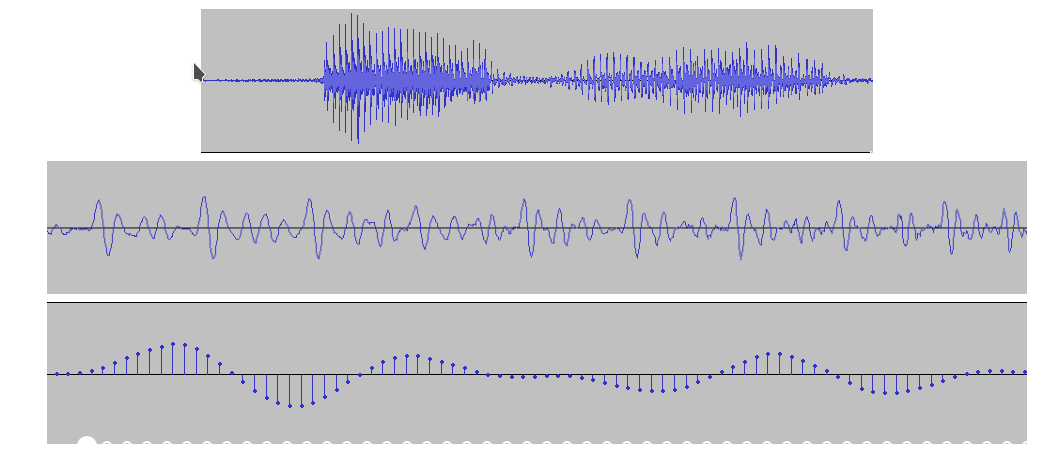
\includegraphics[width=\textwidth]{imagenes/04_01_pcm.png}
\end{figure}

Al hablar de silencio, nos referimos a ausencia total o parcial de sonido, lo cual se puede relacionar directamente con la intensidad de la señal en un segmento de tiempo.

Definiremos intensidad como la sumatoria de las energías en un periodo de tiempo  \cite{Jurafsky2000SpeechRecognition}    

\begin{equation}
\label{eq:energy}
I = \sum{x^2}  
\end{equation}

Esto nos daría un indicador de la toda la señal, sin embargo, es útil realizar este análisis por pequeños segmentos del audio para identificar en conjunto cuales son los puntos donde la intensidad baja representa un espacio de silencio. Estos segmentos por lo general se definen en espacios de 250ms solapados cada 100ms, aunque este solapamiento no es necesario para el proceso de identificación de intensidad, da la idea de que la señal es continua y que cada segmento comparte información con el anterior.

Utilizando esta idea es posible tomar cualquier señal de voz, segmentarla cada 250ms y encontrar los segmentos consecutivos donde la intensidad sea baja o cercana a cero y estos segmentos consecutivos representarían pausas de silencio.

Algunas consideraciones a tomar al usar esta aproximación es que incluso en medio de las señales de voz, existen subsegmentos donde la intensidad es baja, por ejemplo en la pronunciación de consonantes plosivas, como la b, c, d, g, p y t existe una interrupción momentánea y completa del flujo de aire, causando momentáneamente segmentos de silencio.

Usando las anotaciones fonéticas se determinó que la duración promedio de cada consonante plosiva es inferior a los 100ms, también realizando una anotación manual de sonidos y silencios sobre múltiples grabaciones de la anotación por declaración se determinó que los espacios de silencio entre frases eran de mínimo 500ms. De esta manera, utilizando segmentación de 250ms de longitud y desplazamiento de 100ms, se determinan como silencios los conjuntos de segmentos consecutivos de tamaño superior a cinco. 

Entendiendo la condición necesaria para determinar los silencios en una grabación de voz, es posible ejecutar el proceso asumiendo el silencio como ausencia completa de señal, sin embargo, salvo en condiciones muy especiales, donde exista un ambiente libre de ruido, como en un estudio de grabación con filtros físicos, análogos o digitales, en los espacios de silencio la intensidad no es estrictamente cero.

Mas aún, dependiendo de las condiciones y ambiente de grabación, los valores de intensidad en segmentos de silencio varían.

Considerando esto, se propusieron dos aproximaciones para determinar los segmentos de silencio, la primera normalizando los valores de la señal y definiendo un umbral fijo de intensidad en proporción al valor mas alto de la grabación, considerando valores de 0.3, 0.15 y 0.15 que representan umbrales de intensidad del 30\%, 15\%, y 5\%. También se experimentó utilizando algoritmos de agrupamiento con dos centroides iniciales en 0 y la intensidad máxima.

Los resultados se presentan en la tabla \ref{tab:resultados_segmentacion_silencios}

\begin{table}[H]
\centering
\caption{Resultados de la segmentación por silencios}
% \caption{Speech English Corpus}
\label{tab:resultados_segmentacion_silencios}
\begin{tabular}{|l|l|}
\hline
\textbf{Umbral} & \textbf{Precisión}  \\ \hline
Fijo 30\%       & 57.01\%             \\  \hline
Fija 15\%       & 83.26\%             \\  \hline
Fija 5\%        & 69.05\%             \\  \hline
Dinámico        & 74.53\%             \\  \hline
\end{tabular}
\end{table}


\section{Alineación basada en duración de fonemas}

\textcolor{red}{WIP}

Utilizando la segmentación basada en silencios, para determinar cuales son los textos correspondientes se realiza una alineación basada en la duración estimada de un segmento de texto y la duración de los segmentos calculados. Para esto se tomó la anotación fonética para determinar la duración promedio y la desviación estándar de la duración de cada fonema.

Dicha información se puede ver en la tabla \ref{tab:duracion_promedio_fonemas}

\begin{table}[H]
\centering
\caption{Distribución fonética}
\label{tab:duracion_promedio_fonemas}
\begin{tabular}{|l|l|l|}
\textbf{Fonema} &\multicolumn{1}{|p{2cm}|}{\textbf{Duración promedio}} & \multicolumn{1}{|p{2cm}|}{\textbf{Desviación estándar}} \\ \hline
sil & 0.6619 & 0.3700 \\ \hline
a   & 0.1421 & 0.0566 \\ \hline
o   & 0.1487 & 0.0607 \\ \hline
e   & 0.1204 & 0.0416 \\ \hline
n   & 0.1090 & 0.0442 \\ \hline
i   & 0.1294 & 0.0404 \\ \hline
l   & 0.1125 & 0.0530 \\ \hline
s   & 0.1811 & 0.1059 \\ \hline
t   & 0.0784 & 0.0507 \\ \hline
d   & 0.0877 & 0.0536 \\ \hline
R   & 0.0999 & 0.0517 \\ \hline
b   & 0.0826 & 0.0610 \\ \hline
r   & 0.0750 & 0.0254 \\ \hline
p   & 0.0692 & 0.0649 \\ \hline
j   & 0.1038 & 0.0659 \\ \hline
u   & 0.1441 & 0.0507 \\ \hline
m   & 0.1183 & 0.0515 \\ \hline
k   & 0.1224 & 0.0904 \\ \hline
g   & 0.1016 & 0.0970 \\ \hline
f   & 0.1402 & 0.0569  \\ \hline
c   & 0.1032 & 0.0838  \\ \hline
y   & 0.1118 & 0.0044  \\ \hline
C   & 0.1274 & 0.0248  \\ \hline
N   & 0.0575 & 0  \\ \hline
S   & 0.0927 & 0  \\ \hline
\end{tabular}
\end{table}

\section{Segmentación basada en información fonética de formantes en vocales}

\textcolor{red}{WIP}

La manera de entender los sonidos del lenguaje hablado ocurre por por la similaridad de los sonidos emitidos por cualquier locutor. Estas maneras de articular cada fonema permite que todos ellos tengan la misma una composición acústica similar.

Las vocales por ser sonidos de duración promedio mas alta y donde las características que las definen son pocas, únicamente la apertura de cuerdas bocales y la apertura de la boca, permiten que se caractericen utilizando una descomposición acústica.

Al descomponer cualquier señal utilizando la transformada de Fourier

\begin{equation}
\label{eq:fourier}    
f(x) = \frac{1}{2} \, a_{0} + \sum_{n=1}^{\infty} \left[
   a_{n}\,\boldsymbol{\cos} (n\,x) + b_{n} \,\boldsymbol{\sin} (n\,x) \right]
\end{equation}

Se obtienen señales raíz de cada onda compleja. Con las señales de voz, los coeficientes máximos  en el orden ascendente de la frecuencia se denominan formantes, y el formante 1 (f1) y el formante 2 (f2) representan efectivamente el fenómeno efectuado por las cuerda vocales vibrando y la resonancia dad por la cavidad bucal.

Para el idioma español los formantes teóricos para el español se muestra en la tabla \ref{tab:formantes_teoricos}, los cuales fueron tomados a partir locutores con dialecto peninsular y donde se muestra la distribución vocálica incluyendo los dos primeros formantes \cite{Bradlow1995}.

\begin{table}[H]
\centering
\caption{Formantes teóricos para vocales del español.}
\label{tab:formantes_teoricos}
\begin{tabular}{|l|l|l|l|l|}
\hline
\textbf{Vocal} & \textbf{f1} & \textbf{f2} & \textbf{std f1} & \textbf{std f2} \\ \hline
a   & 638 & 36 & 1353 & 84 \\ \hline
e   & 458 & 42 & 1800 & 131 \\ \hline
i   & 286 & 6  & 2200 & 131 \\ \hline
o   & 460 & 19 & 1019 & 99 \\ \hline
u   & 300 & 20 & 992  & 121 \\ \hline

\end{tabular}
\end{table}

También se realizó una observación de las vocales calculando sus formantes basados en la información extraida de las palabras anotadas fonéticamente. Esta información se encuentra en la tabla \ref{tab:formantes_observador} 

\begin{table}[H]
\centering
\caption{Formantes teóricos para vocales del español}
\label{tab:formantes_observador}
\begin{tabular}{|l|l|l|l|l|}
\hline
\textbf{Vocal} & \textbf{f1} & \textbf{f2} & \textbf{std f1} & \textbf{std f2} \\ \hline
a   & 682.84 & 1347.66 & 73.77 & 93.04 \\ \hline
e   & 494.84 & 1619.97 & 55.49 & 132.84\\ \hline
i   & 382.33 & 1657.33 & 50.65 & 155.24 \\ \hline
o   & 506.24 & 1101.14 & 60.20 & 170.64\\ \hline
u   & 434.77 & 984.185 & 50.32 & 193.66\\ \hline

\end{tabular}
\end{table}

A partir de esta información se realizaron experimentos buscando la precisión en la identificación de las vocales, tomando una distancia L1 de los dos primeros formantes y aumentando un umbral definido fijo y también utilizando la desviación estándar sobre los formantes observados. Adicionalmente a esto se entrenó un algoritmo de agrupación no supervizado K-means inicializando los centroides en los formantes observados. Los resultados se reportan en la tabla \ref{tab:resultados_vocales}

\input{tablas/04_05_segmentación_vocalica}


Para entender los bajos resultados presentados por la aproximación basada en los formantes observados y su desviación, se graficó sobre grabaciones con contenído de solo las vocales, graficando los formantes 1 y 2 en espacios donde la intensidad superaba los 60 decibeles y graficando también los formantes observados y su desviación estándar de las vocales a en la figura \ref{img:formantes_a} y e en la figura \ref{img:formantes_e}

\begin{figure}[H]
\caption{Formantes de vocal A}
\label{img:formantes_a}
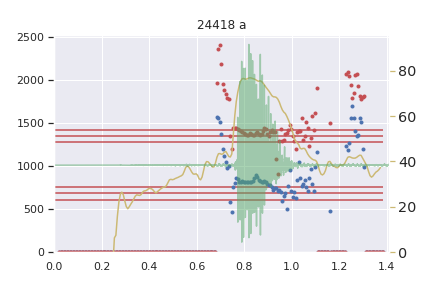
\includegraphics[width=\textwidth]{imagenes/04_02_a.png}
\end{figure}

\begin{figure}[H]
\caption{Formantes de vocal E}
\label{img:formantes_e}
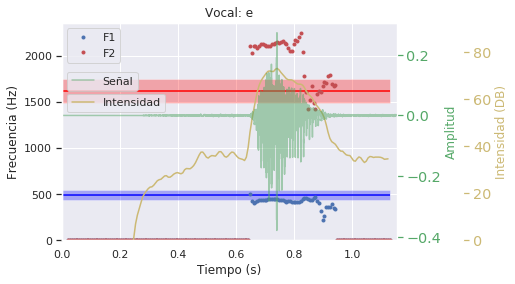
\includegraphics[width=\textwidth]{imagenes/04_02_e.png}
\end{figure}

En ambas figuras se muestra en verde la onda, en azul el formante 1 en rojo el formante dos, en amarillo la intensidad cuyo valor se encuentra en el eje derecho y en rojo y azul claro los rangos esperados siendo la línea centra el formante observado promedio y las lineas adyacentes los valores de sumar y restar la desviación entándar.

Como se observa en la grabación de la letra e, hay un ambiente mas ruidoso, lo que hace que se capturen valores de formantes en lugares donde aún no hay señal de voz y aunque en los momentos donde la señal se estabiliza, los formantes tienden a acercarse a las bandas de frecuencia esperadas, esto no ocurre en todos los casos.